%%% LyX 2.0.5.1 created this file.  For more info, see http://www.lyx.org/.
%%% Do not edit unless you really know what you are doing.
%\documentclass[twoside,english]{report}
%\usepackage[T1]{fontenc}
%\usepackage[latin9]{inputenc}
%\setcounter{secnumdepth}{3}
%\setcounter{tocdepth}{3}
%\usepackage[active]{srcltx}
%\usepackage{verbatim}
%\usepackage{graphicx}
%\usepackage{setspace}
%\usepackage[numbers]{natbib}
%\doublespacing
%
%\makeatletter
%
%%%%%%%%%%%%%%%%%%%%%%%%%%%%%%% LyX specific LaTeX commands.
%\providecommand{\LyX}{L\kern-.1667em\lower.25em\hbox{Y}\kern-.125emX\@}
%%% Because html converters don't know tabularnewline
%\providecommand{\tabularnewline}{\\}
%
%\makeatother
%
%\usepackage{babel}
%\begin{document}

\chapter{Introduction}

\section{Problem Definition}

The growing use of keyboard-less handheld devices accelerates a transition in the Human-Computer data input interface.  While in the past, keyboards and mice were the primary mode of data entry, nowadays, hand and finger gestures are increasingly used for this task. Consequently, a growing interest in the online character recognition field has taken place. Automated script recognition of Latin, Chinese and Kanji has been a focus of study in the last decade and impressive recognition rates were achieved. However, Arabic text recognition is at an early stage. The reason for this is lack of funds and other utilities such as text database, dictionaries, etc. [2]
Text recognition can be classified into two main fields: online and offline recognition. Online recognition aims recognizing the text as it is being written. However, in the offline script recognition field, a digital image containing text is fed to the computers and the system attempt to recognise the written text [3]. The main existing approaches for script recognition are the holistic approach and the analytic approach. The holistic approach considers the global properties of the written text while the analytic approach involves segmentation and classification of each part of the text. 
Arabic text, both handwritten and printed is cursive. An Arabic word consists of one or more sub-words (which will be referred to as word parts). Each word part consists of one character or more. Thus, most of the online Arabic recognition systems perform the recognition soon after the word part scribing is completed using the holistic or the analytic approach. The analysis of Arabic script is further due to obligatory dots and stokes that are placed above or below most letters in addition to the wide range variety of writing fashions.
In this thesis we propose a novel approach which combines both holistic and analytic techniques for recognizing open dictionary Arabic online script. The recognition process, in our approach, is performed whilst the word part is being written. At the first stage, demarcation points are identified using SVM. At the second stage we employ an agile but loose classifier to select letters candidates for each segment. Finally, we holistically recognize the word part by applying a costly yet accurate classifier. 

\emph{see: \cite{al2010development} for a well written introduction}


\section{Approach Overview}

While the holistic approach is a common technique used for Arabic handwriting recognition, this approach is not practical for recognizing words from the unrestricted dictionary (contains all the words in the Arabic dictionary), since it needs to train the system for each word in the dictionary.  As mentioned in section 2.2 there are about 40,000 valid word parts, with different main strokes. There are much more classes if additional strokes are taken into consideration, practically, a very large number of classes. To overcome this problem, we propose an Arabic word-parts recognizer which breaks up the whole recognition process to 2 restricted recognition tasks. The first is analytical letters classification and the other is holistic word-part recognition from the limited dictionary that contains veritable combinations of letters candidates found in the previous stage. The most significant benefit of this approach is that in both stages the recognition is performed on spaces which contain a very limited class number. 


In this section we draw the skeleton of our recognition process. Figure \ref{fig:overview} presents the main flow of our approach followed by a brief description on each stage.

\begin{figure}
\centering
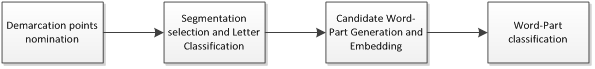
\includegraphics{./figures/overview}       
\caption{The main stages of the recognition system.}
\label{fig:overview}
\end{figure}

\subsection{Demarcation Points Nomination}
The goal of this stage is to decide coarsely but effectively if a certain point is a demarcation point. This stage is performed while the word part is being written. To identify demarcation point we have used the following 2 Arabic demarcation points characteristic: 1. Demarcation point lives in a horizontal region. 2. Demarcation point is usually contained in a Forward region. More details and definitions will follow in a section \emph{[]}. We present a novel algorithm online segmentation using static rules engine. Over segmentation and under-segmentation are the main problems segmentation algorithms encounter. Over segmentation is handled in the next stage. Under-segmentation is handled by a defining a new notion named hyper-letter, which represents combinations of letters that the demarcation points between them is sometimes concealed. More details will be given in section \emph{[]}.

\subsection{Segmentation selection and Letter classification}
This stage starts when the user finishes to scribe the stroke, i.e. on "pen up" event.  The goal of this sub-process is to select the set of demarcation points which gives the best letter recognition results. This is done after the writer has completed scribing the main body of the stroke. Segmentation induces partition to subsequences, where each subsequent is a geometric representation of a letter (or a combination or letters). The subsequence is classified to a set of 3 or candidate letters using a combination of EMD and DTW metrics. The quality scoring of the segmentation is based on the recognition score of each letter which is calculated using dynamic programming technique. 

\subsection{Candidate Word-Part generation and embedding}
After the segmentation is determined and each sub-sequent was classified to a small set of hyper-letters candidates, the system generate all possible word-parts sequences using the samples of hyper-letters in our letters database using the most common ways to write the hyper-letter. Here we use the Holistic approach to classify the word-part. However, instead of taking the whole dictionary of possible word-parts, our space of candidate word part only samples of word parts combinations of letters nominated in the previous stage. Subsequently, we extract the features of the generated word-parts and embed them using approximate Earth Movers Distance (EMD) approach described by Shirdhonkar and Jacobs in \cite{shirdhonkar2008approximate}.

\subsection{Candidate Word-Part generation and embedding}
The number of possible different word-parts is relatively small. Assume that the written word part composed of 4 letters. For every letter, the second stage has nominated 3 different letters. In the worst case when all combinations are legal, we get at most $3^4=27$ different possible word-parts. However, the number of different samples created is very large. Thus, we need a fast classification approach to overcome this obstacle. 
EMD is a true metric, thus we can utilize a recently developed tool which allow fast (sub linear time) approximate nearest neighbor (NN) named Linear Sensitivity Hashing (LSH) presented by Gionis et al in \cite{gionis1999similarity}. LSH indexes a set of training examples living in a normed space by a number of hash tables, such that the probability of collision is high for similar examples and low for dissimilar ones. In this stage, the system initializes an LSH data structure with the set of word parts generated in the previous stage and use it to efficiently find the most similar word-parts.

\section{Notes and Limitations}
As mentioned before, Arabic is a cursive written language and it contains about 40k possible word parts. By "possible", we mean that there is an Arabic word which contains the word part. Arabic letters may differ by additional stroke above or beneath the main stroke. For example, the Arabic letter \RL{f} (Fa) contains a single dot above the main stroke, however the letter \RL{q} (Qa), contains double dots, both having identical main body. In our work we recognize and classify the main body of the letter and ignore the additional stroke entirely. As a result, the number of different letters drops from 29 to18 and the number of different possible word parts decreases to []. It is important to comment that taking the additional strokes into consideration may be exploited to boost the classification rate.
The Arabic letters system contain 7 sets of letters that have the same body, and are differentiated only by the additional strokes above or under it. The following table describes the sets of similarity:

\begin{table}[h]
\caption{Arabic letters shapes similarities}
\begin{tabular}{ | c | c |}
\hline
Letter Set & Positions of similarity\\
\hline                 
  \RL{b}, \RL{t}, \RL{_t} & All Positions\\ 
  \hline
  \RL{`}, \RL{.g} & All Positions\\
  \hline
  \RL{.h}, \RL{j}, \RL{x} & All Positions\\
  \hline
  \RL{f}, \RL{q} & All Positions (very slight differences\\ 
   					&in Isolated mode, the valley of the letter \RL{q} is deeper)\\
  \hline
  \RL{r}, \RL{z} & Isolated\\
  \hline
  \RL{h}, \RL{T} & Isolated\\
  \hline
\end{tabular}
\centering
\label{table:letters_similarity} 
\end{table}

The main body of most Arabic letters is written by a single stroke. However, there are some letters that usually written using 2 strokes, such as the letter \RL{-k-}  which is the middle form of the letter \RL{k} (Ka). The writer usually writes \RL{-l-} and adds the final upper slanted line when the main body is completed, as if he writes an additional stroke.
Another problem arises when trying to recognize Arabic transcript, is that, different writers may write the main body of the same word part in a different number of strokes. For instance, the main body of the word part \RL{byt} (Bayt - Home), is usually written in a single stroke however, sometimes it may be written by some writers using 3 strokes.
We have also considered the common combination of the letter \RL{l} followed by the vowel \RL{A} as a single letter which is commonly drawn as \RL{lA}. 
Also, three consequent appearances of the letter \RL{-b-} (B) in the middle of the word-part looks as follows: \RL{-bbb-}. As can be seen very similar to the \RL{s} (S) letter in its medial position \RL{-s-}, the only to distinguish between the two options is by looking at the additional strokes.
For these mentioned complexities, when recognizing Arabic scripts, most researches have preferred the holistic approach. 



\section{Our Results}

\section{Organization of Thesis}

%\end{document}
